\documentclass{TIJMUjiaoanLL}
\pagestyle{empty}


\begin{document}


%课程名称
\kecheng{系统生物学}
%课程内容
\neirong{转录组学(RNA-Seq数据分析)\ /\ 第3章}
%教师姓名
\jiaoshi{伊现富}
%职称
\zhicheng{讲师}
%教学日期(格式:XXXX年XX月XX日XX时-XX时)
\riqi{2017年3月8日8:00-10:00}
%授课对象(格式:XXX系XXXX年级XX班(硕/本/专科))
\duixiang{生物医学工程与技术学院2014级生信班(本)}
%听课人数
\renshu{30}
%授课方式
\fangshi{理论讲授}
%学时数
\xueshi{2}
%教材版本
\jiaocai{系统生物学,第1版}


%教案首页
\firstHeader
\maketitle
\thispagestyle{empty}

\mudi{
\begin{itemize}
  \item 掌握Tuxedo套装的组成工具及各自的作用与使用方法。
  \item 熟悉RNA-Seq数据分析的常用工具。
  \item 了解RNA-Seq的在科学研究中的实际应用。
  \item 自学RNA-Seq数据分析工具的使用方法。
\end{itemize}
}

\fenpei{
\begin{itemize}
  \item (5')引言与导入:回顾RNA-Seq的基本流程。
  \item (30')RNA-Seq数据分析:根据RNA-Seq的数据分析流程,简单介绍每个步骤的常用工具。
  \item (40')Tuxedo套装:介绍RNA-Seq数据分析的Tuxedo套装,介绍组成套装的工具,讲解各自的作用与使用方法。
  \item (20')RNA-Seq应用实例:根据文献报道,介绍RNA-Seq在差异表达分析、融合基因检测等方面的实际应用。
  \item (5')总结与答疑:总结授课内容中的知识点与技能,解答学生疑问。
\end{itemize}
}

\zhongdian{
\begin{itemize}
  \item 重点:RNA-Seq数据分析的常用工具,Tuxedo套装的使用。
  \item 难点:Tuxedo套装的使用。
  \item 解决策略:通过实例讲解和比较类比帮助学生理解、记忆。
\end{itemize}
}

\waiyu{
  \vspace*{-10pt}
  \begin{multicols}{2}
    质量控制(quality control)

    多重检验(multiple test)

    基因集(gene set)
  \end{multicols}
  \vspace*{-10pt}
}

\fuzhu{
\begin{itemize}
  \item 多媒体:RNA-Seq数据分析的常用工具,RNA-Seq的应用实例。
  \item 板书:RNA-Seq数据分析流程,Tuxedo套装。
\end{itemize}
}

\sikao{
  \vspace*{-10pt}
  \begin{multicols}{2}
  \begin{itemize}
    \item 总结RNA-Seq数据分析的基本流程。
    \item 列举RNA-Seq数据分析的常用工具。
    \item 解释RNA-Seq数据分析中的Tuxedo套装。
    \item 总结Tuxedo套装的使用方法。
  \end{itemize}
  \end{multicols}
  \vspace*{-10pt}
}

\cankao{
\begin{itemize}
  \item 维基百科等网络资源。
\end{itemize}
}

\firstTail


%教案续页
\newpage
\otherHeader

\begin{enumerate}
  \item 引言与导入(5分钟)
    \begin{itemize}
      \item RNA-Seq实验流程:RNA $\Rightarrow$ Fragement $\Rightarrow$ cDNA $\Rightarrow$ PCR $\Rightarrow$ Sequencing
      \item RNA-Seq分析流程:QC $\Rightarrow$ Preprocessing $\Rightarrow$ Mapping $\Rightarrow$ Assembly $\Rightarrow$ DE
    \end{itemize}

  \item \textcolor{red}{【重点】}RNA-Seq数据分析(30分钟)
    \\ \textcolor{red}{结合RNA-Seq的分析流程介绍工具及其作用}
    \begin{enumerate}
\parpic[fr]{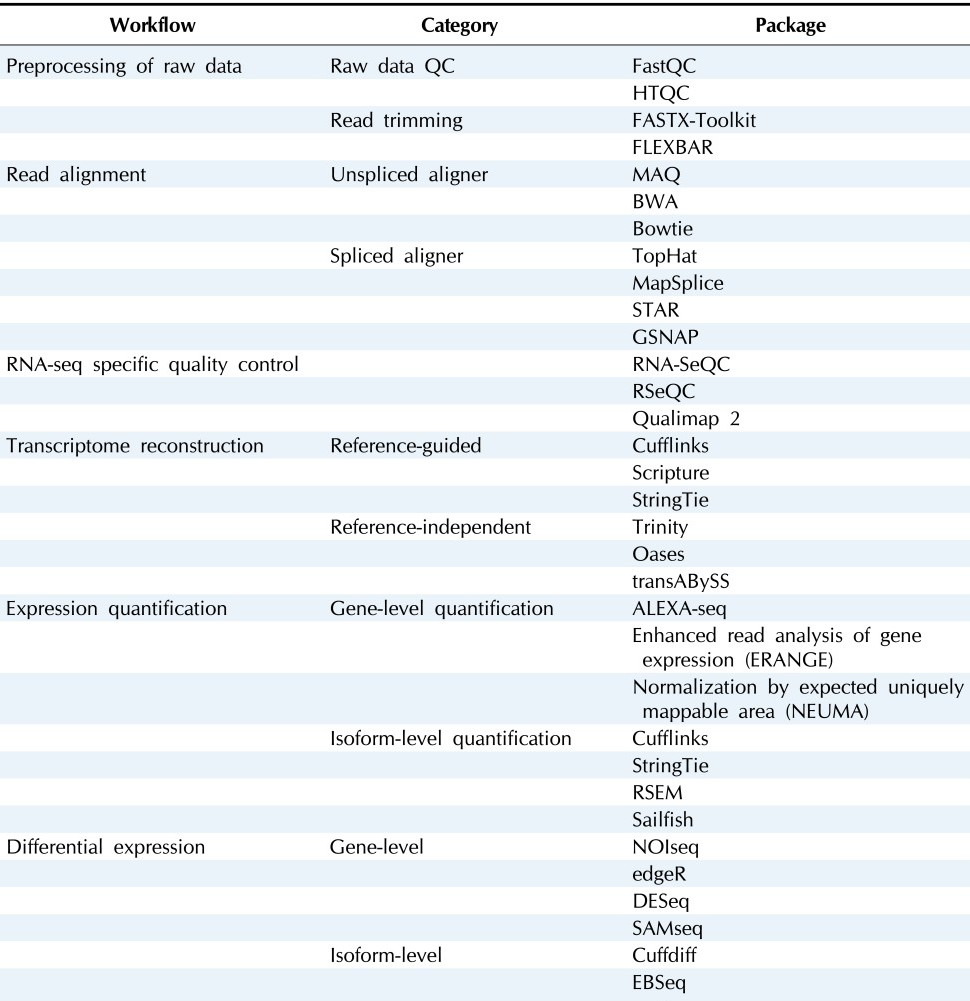
\includegraphics[width=7.8cm]{c3_tool_pipeline_01.jpg}}
      \item Quality control: FastQC, NGSQC, RNA-SeQC, RSeQC
      \item Trimming and adapters removal: FASTX Toolkit, PRINSEQ, cutadapt
      \item Alignment: TopHat
      \item Transcriptome assemble: Cufflinks, Scripture
      \item Expression: Cufflinks, DESeq, EdgeR, DEGseq, baySeq
      \item Workbench: easyRNASeq, Galaxy, GenePattern, Taverna
      \item Visualization: ngs.plot, GBrowse, IGB, IGV, SeqMonk, Tablet
      \item Databases: ENCODE, RNA-Seq Atlas, SRA
    \end{enumerate}


  \item \textcolor{red}{【重点,难点】}Tuxedo套装(40分钟)
    \\ \textcolor{red}{结合RNA-Seq的分析流程进行讲解}
    \begin{enumerate}
      \item Tuxedo简介\textcolor{red}{(讲解每个工具的作用及相互之间的联系)}
        \begin{enumerate}
\parpic[fr]{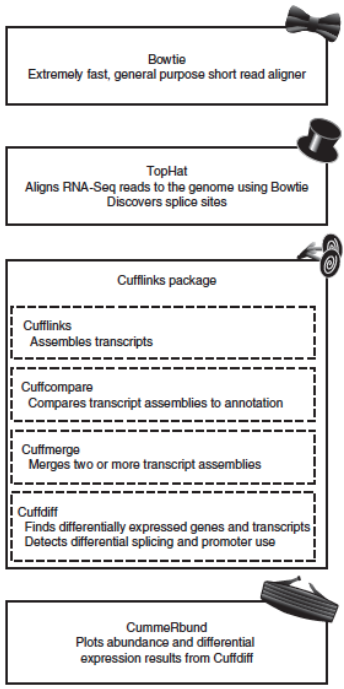
\includegraphics[width=4cm,height=10cm]{c3_tool_tc_00.png}}
          \item Bowtie: Ultrafast short read alignment
          \item TopHat: Aligns RNA-Seq reads to the genome using Bowtie; Discovers splice sites
          \item Cufflinks package
            \begin{itemize}
              \item Cufflinks: Assembles transcripts
              \item Cuffcompare: Compare transcript assemblies to annotation
              \item Cuffmerge: Merges two or more transcript assemblies
              \item Cuffquant: Compute the gene and transcript expression profiles
              \item Cuffdiff: Finds differentially expressed genes and transcripts;\\ Detects differential splicing and promoter use
              \item Cuffnorm: Normalize the expression levels from a set of\\ samples to be on as similar scales as possible
            \end{itemize}
          \item CummRbund: Plots abundance and differential expression results from Cuffdiff
        \end{enumerate}
      \item Tuxedo使用\textcolor{red}{(结合工具之间的关联讲解套装的使用)}
        \begin{figure}[h]
          \centering
          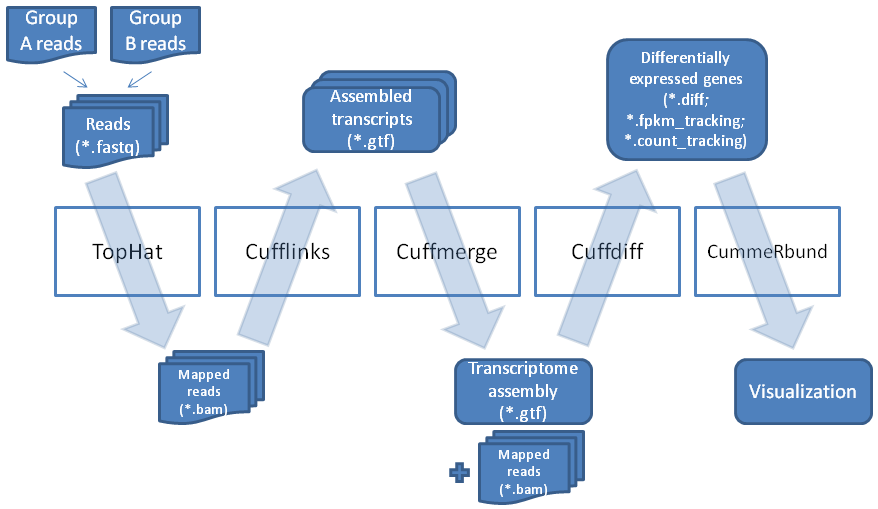
\includegraphics[width=0.45\textwidth]{c3_tool_tc_04.png}
          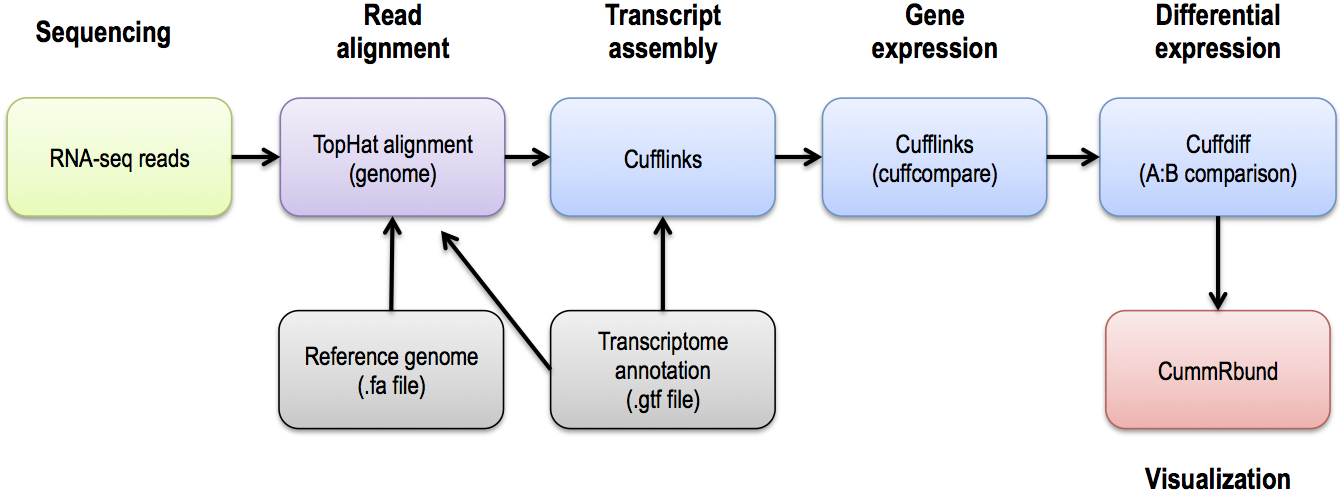
\includegraphics[width=0.5\textwidth]{c3_tool_tc_03.png}
        \end{figure}

\otherTail
\newpage
\otherHeader

      \item 补遗
        \begin{itemize}
% \parpic[fr]{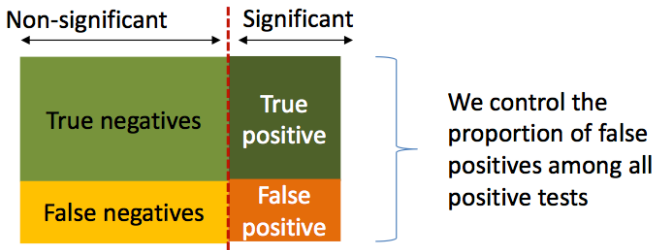
\includegraphics[width=8cm]{c3_workflow_test_01.png}}
          \item Multiple test: p-value vs. FDR
          \item Downstream analysis: DAVID, GSEA, GO, KEGG
        \end{itemize}
        \begin{figure}[h]
          \centering
          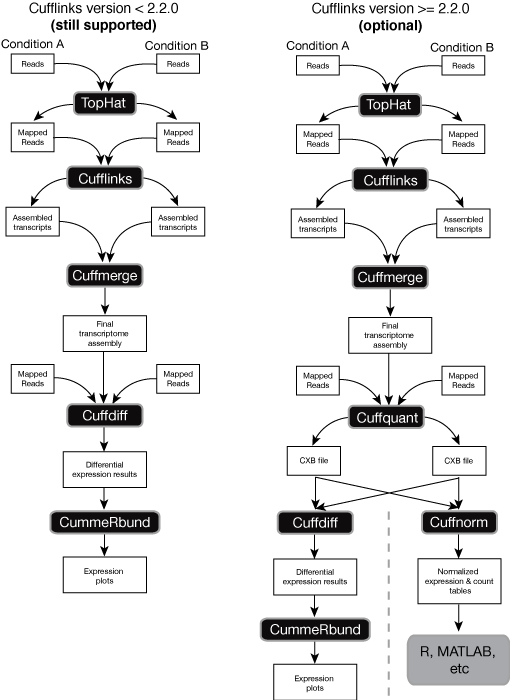
\includegraphics[width=0.8\textwidth]{c3_tool_tc_01.png}
        \end{figure}
    \end{enumerate}

  \item RNA-Seq应用实例(20分钟)
  \begin{multicols}{3}
    \begin{itemize}
      \item DGE
      \item Fusion gene
      \item Splice variant
      \item Novel transcript
      \item lncRNA
      \item miRNA
      \item Alternative promoter use
    \end{itemize}
  \end{multicols}

\otherTail
\newpage
\otherHeader

  \item 总结与答疑(5分钟)
    \begin{enumerate}
      \item 知识点
	\begin{itemize}
    \item RNA-Seq数据分析:基本流程,常用工具
	  \item Tuxedo套装:组件,作用,使用方法
    \item RNA-Seq应用实例:DGE,Fusion gene,…
	\end{itemize}
      \item 技能
	\begin{itemize}
    \item 掌握RNA-Seq数据分析常用工具的使用方法
    \item 使用Tuxedo套装分析RNA-Seq数据
	\end{itemize}
    \end{enumerate}
\end{enumerate}

\otherTail


\end{document}

